\label{axon200commander}

\begin{figure}[h]
\begin{center}
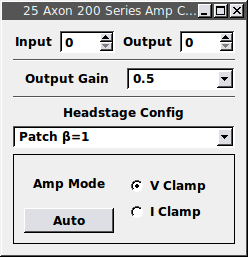
\includegraphics[width=2in]{axon200.png}
\caption[axon200]{Control module for Axon 200 Series Amplifier Commander.}
\end{center}
\end{figure}

Tested with the 200A and 200B, the Output Gain, Headstage Config, and Amp Mode must match the amplifier settings set by its switches. The module is able to sense the mode through the amplifier's mode telegraph, located on the back of the amplifier.

input(0) - "Mode Telegraph" : The analog voltage signal from the amplifier corresponding to the mode of the amplifier.